\section{Database Model for Storing OSA Data}
A database for storing Obstructive Sleep Apnea related data is discussed in the thesis "An open database model for storing Obstructive Sleep Apnea data" by Viet Thi Tran \cite{viet}. The thesis presents the design and implementation of a relational \textit{database model} for \textbf{storing} OSA signals and bio-physiological signals, simplify the \textbf{analysis} of the signals, and supporting acquisition from \textbf{future data sources}. 

In terms of storing data in a database system, the context of what the database is used for, and what it must contain, are usually crucial to identify the appliance of the database. For storing OSA related data, the database system must satisfying the requirements of the sensor sources, and requirements of the users of the system. The users in the system are \textit{patients, physicians, and researchers}. A few characteristics of the actions the users can take are:
\begin{enumerate}
    \item \textit{Patients} -- the users of the group are able to execute a simple function (i.e. inserting, deleting and queries). Such function might be finding records, storing sample from CESAR tool, and import/exporting certain recordings. Mostly, their action are to import and to export. 
    \item \textit{Physicians} -- are able to apply functions that modify existing data, manually training data for a recording, retrieve all recording of patients, etc... In other words, they have knowledge of OSA health data and may tweak values based on their expertise in the field.
    
    % [Fix first sentence]
    \item \textit{Researchers} -- often evaluates tasks on the system to find the best solution. Thus, they would most likely want to evaluate the quality of the source that is used for collecting the signals. Some actions they can take are to evaluate quality of sources and channels, perform raw query to find a cost and performance beneficial query, and applying possible mining algorithms. 
\end{enumerate}

The benefits of using a relational database to store the OSA related signals are: \textit{data analysis} can be performed on client's device (e.g. mobile devices) by utilizing SQL and its supporting algorithms; \textit{remote services} to fetch parts of the client's data by using remote querying; and \textit{privacy of patients} is not violated as the data remains on their devices and they can decide which data they would like to share. 

%Systems can be defined by functional and non-functional requirements. Functional requirements are statements of services the system should provide, whilst non-functional requirements are constraints on the service or functions offered by the system. For the database of the system, the functional requirements are:
%\begin{enumerate}
%    \item The application must reuse CESAR acquisition tool to collect data from BITalion.
%    \item The application must support importing and exporting EDF files.
%    \item Data analysis can be performed by using the application.
%    \item Collected data could be visualized in real-time data, or replay from the stored data.
%    \item Annotations could be added manually to a certain source
%\end{enumerate}


A logic data model describes the abstract structure of the database system without considering physical structure, i.e., how the database is implemented. The features of a logical data model includes: \textit{tables (entities)} and all relations between them; \textit{columns (attributes)} for the entities; \textit{primary key} for all of the entities; and \textit{foregin key} for identifying relations between different entities. 

Before analyzing the proposed data model of the system, we identify the entities that are part of the system:
\begin{itemize}
    \item \textbf{Source} -- is the entity storing the data obtained from CESAR acquisition tool, in addition to EDF files. Mainly, the entity stores the bio-signals data from sensor sources (such as BiTalino). 
    \item \textbf{Recording} -- is a session of sample recorded on the \textit{users} device. 
    \item \textbf{Person} -- is both the \textit{Patient} and the \textit{Physician} (however, I could not find any listing of \textit{Researchers} in the thesis), because these two entities share common attributes. 
    \item \textbf{Clinic} -- provides advanced diagnostic or treatment services for specific diseases. The bio-physiological signals are usually stored in formats tailored specific to a
clinic. Thus, the clinics have their own way of formatting and manipulating the
bio-physical signals to their standards, and the data may be varying
between clinics.
\end{itemize}

The actual data model, we can define the relationship between the entities based on the identified requirements. In Figure \ref{fig:modelrelations}, we have a logical data model for the entities in the system, based on the following relations:
\begin{enumerate}[label=\alph*)]
    \item Each Source has many Recordings, but one Recording belongs to only one Source.
    \item Each Source can be used by many different Persons, and each Person can use many different Sources.
    \item Each Source can be used by many different Clinics, and each Clinic can use many difference Sources.
    \item Person has many Recordings, but one Recording belongs to only one Person.
    \item Person collects many Recording, but one Recording is collected by only one Person.
    \item Each Recording is produced by a Source, for a Person at a certain Clinic at a certain time.
    \item Each Person works/belongs to many Clinics, and each Clinic employs/has many Persons.
    \item Each Person (Physician) observe many Persons (Patient), and many Person (Patient) are observed by a Persons (Physician).
\end{enumerate}

\begin{figure}[ht]
    \centering
    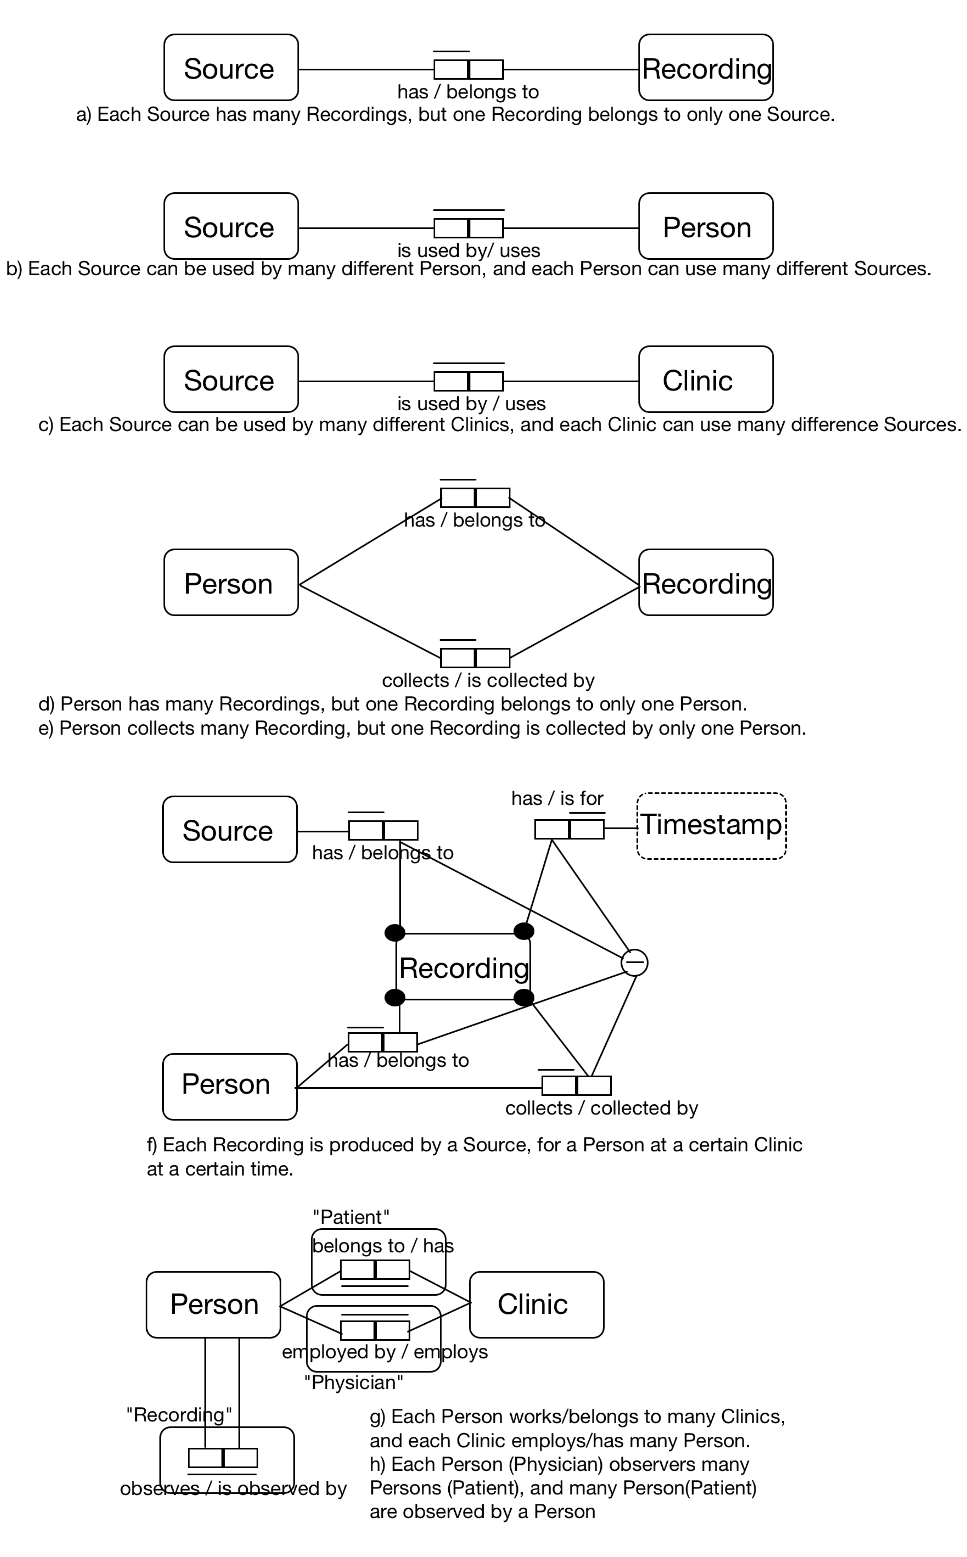
\includegraphics[width=0.94\textwidth]{images/Group.png}
    \caption{Binary, recursive and n-ary relationships \cite{viet}}
    \label{fig:modelrelations}
\end{figure} 


Normalization is a technique in relational database used for integrity, maintainability and performance of database. The purpose is to reduce the redundancy of the data stored in a database system, so the database can become more reliable and efficient.  The table of data can be classified on: (1NF) first normal form; (2NF) second normal form; (3NF) third normal form; (BCNF) Boyce-Codd normal form; and (4NF) fourth normal form. Where a higher degree of a normal form is preferable.

In the thesis, the entities (source, recording, person, and clinic) of the system have their normal form evaluated by determining the functional dependencies and the multivalued dependencies based on the attributes of the entity. The normal form can then be derived by applying set of algorithms and rules (i.e., determining the normal form of the FDs/MVDs and decomposing it until the tables is on BCNF/4NF). By doing this, we ensure the data to be loss less on joins, in addition to reducing the redundant storage. The end result of the following steps, splits some of the entities into smaller groups of entities with common attributes:

%\begin{center}
%    \textit{Source} \textrightarrow{} \textbf{Sensor Source} and \textbf{Channel}
%    
%    \textit{Person} \textrightarrow{} \textbf{Person}, \textbf{Patient} and \textbf{Physician}
%    
%    \textit{Recording} \textrightarrow{} \textbf{RecordAnnotation}, \textbf{Annotation}, \textbf{Record} and \textbf{Sample}
%\end{center}

The final result of the logical data model is presented in Figure \ref{fig:Figures/LogicalModelDB1} and \ref{fig:Figures/LogicalModelDB2}. Theoretically, the model can be implemented and deployed on a database management system, which then can be used to store Obstructive Sleep Apnea data.

\begin{figure}
    \centering
    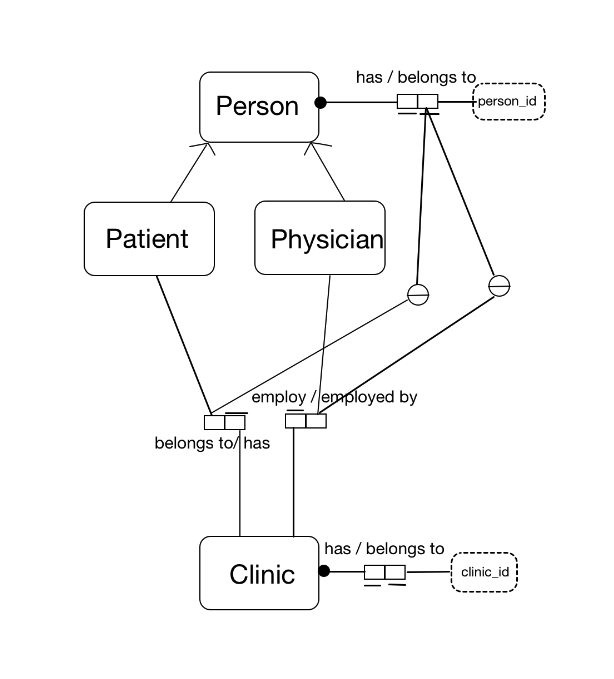
\includegraphics[width=1.0\textwidth]{images/LogicalModelDB1.png}
    \caption{Logical model of the OSA database - Person and Clinic \cite{viet}}
    \label{fig:Figures/LogicalModelDB1}
\end{figure}
\begin{figure}
    \centering
    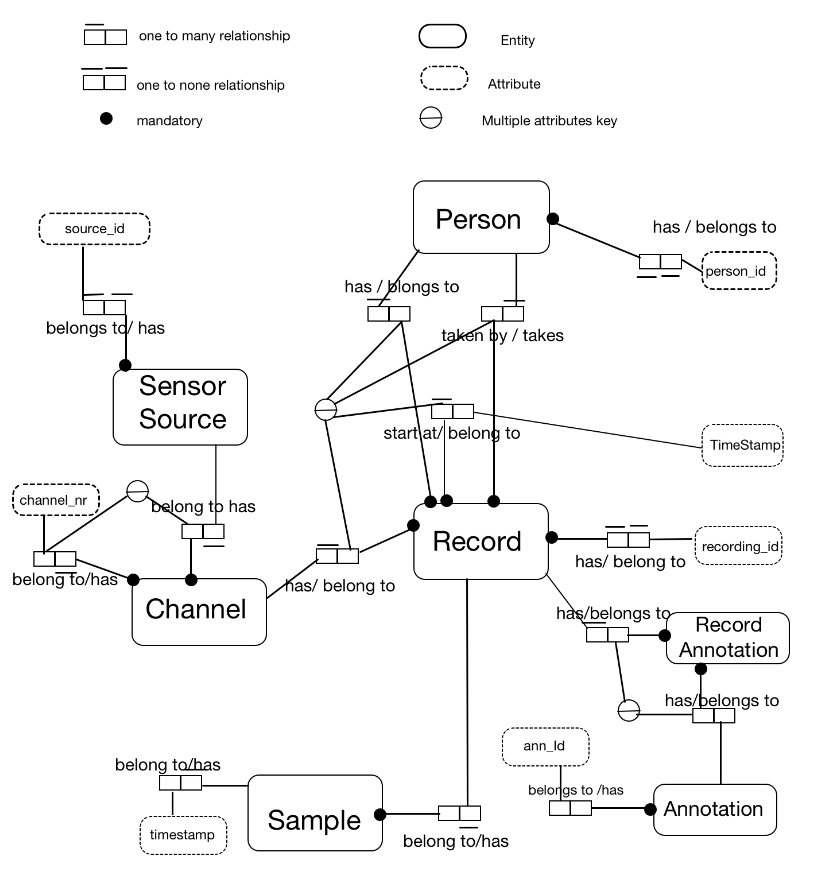
\includegraphics[width=1.0\textwidth]{images/LogicalModelDB2.png}
    \caption{Logical model of the OSA database - Source and Recording \cite{viet}}
    \label{fig:Figures/LogicalModelDB2}
\end{figure}